\documentclass[12pt, a4paper, oneside]{ctexart}
\usepackage{amsmath, amsthm, amssymb, graphicx}
\usepackage[bookmarks=true, colorlinks, citecolor=blue, linkcolor=black]{hyperref}
\usepackage[margin = 25mm]{geometry}
\usepackage{setspace}
\usepackage{listings}
\usepackage{cite}
\usepackage{ctex}
\usepackage{float}
\usepackage{xcolor}

\definecolor{codegreen}{rgb}{0,0.6,0}
\definecolor{codegray}{rgb}{0.5,0.5,0.5}
\definecolor{codepurple}{rgb}{0.58,0,0.82}
\definecolor{backcolour}{rgb}{0.95,0.95,0.92}

\lstdefinestyle{mystyle}{
    backgroundcolor=\color{backcolour},   
    commentstyle=\color{codegreen},
    keywordstyle=\color{magenta},
    numberstyle=\tiny\color{codegray},
    stringstyle=\color{codepurple},
    basicstyle=\ttfamily\footnotesize,
    breakatwhitespace=false,         
    breaklines=true,                 
    captionpos=b,                    
    keepspaces=true,                 
    numbers=left,                    
    numbersep=5pt,                  
    showspaces=false,                
    showstringspaces=false,
    showtabs=false,                  
    tabsize=2
}

\lstset{style=mystyle}


\title{WKB近似方法在非均匀密度等离子体中的波传播问题}
\date{\today}
\author{202011010101物理2001孙陶庵}
\begin{document}
\begin{spacing}{2.0}
\tableofcontents
\maketitle

\section{引言}
量子物理中的WKB(Wentzel-Kramers-Brillouin)近似是一种强大的工具,用于解决薛定谔方程的近似解。
WKB近似基于波函数的相位变化和振荡特性,通过将波函数表示为相位和振幅的乘积形式,将量子力学问题转化为经典力学的问题。
该近似方法适用于存在明显变化的势能场或介质中的波的传播。

该方法在描述均匀介质中的量子现象和波动行为方面具有广泛的应用。然而,许多实际系统,如非均匀等离子体,具有空间上的变化性质,
导致了更为复杂的物理行为。在这种情况下,我们需要将WKB近似扩展到非均匀介质,以更准确地描述系统的性质和行为。

在散射截面研究方面,WKB近似提供了一种计算总散射截面的有效方法。通过利用WKB近似,我们可以将散射问题转化为经典轨迹的求解,
从而得到散射截面的近似解析表达式。这种方法不仅可以用于分析单个散射体的散射特性,还可以推广到多体系统和复杂散射体的情况。

在非均匀等离子体中,WKB近似也被广泛应用于描述非均匀等离子体中的波的传播和能量吸收过程。等离子体是由离子和自由电子组成的带电气体,
然而,由于等离子体密度、温度和电场等物理量在空间上的变化,非均匀等离子体的性质和行为比均匀介质更为复杂和多样化。
WKB方法在等离子体物理中是非常有价值的解决方案,因为这个方法提供了一个直观的方式描述波的传播;
通过一个局部色散关系定义的波,其幅度和相位以一种非常明显的方式与这种局部的特征相关

本文将首先介绍WKB近似的基本原理和物理意义,然后探讨其在散射截面研究和等离子体物理中的具体应用。通过深入理解和应用WKB近似,
我们将能够更好地解释和分析散射现象以及等离子体中的波动行为。


\section{WKB近似的基本原理}
WKB(Wenzel,Kramers, Brillouin)方法是得到一维定态 Schrödinger 方程的近似解的一种技术,
其基本思想同样可应用于许多其他形式的微分方程和三维 Schrödinger 方程的径向部分,其最基本的核心思想主要是:
首先波函数以指数函数的形式重新表达,再将这指数函数代入Schrödinger方程,展开指数函数的参数为$\hbar$的幂级数,
$\hbar$同次幂的项目一一对应,会得到一组方程,处理后,就会得到波函数的近似。
\subsection{基本思想}
中间省略了很多步骤,详细过程参见各大量子力学课本\cite{griffiths_schroeter_2018},以及这篇文章皆有非常好的讲解\cite{LU2018502}
对于一维定态Schrödinger方程:
\begin{center}
    $\displaystyle - \frac{\hbar^2}{2m} \frac{\mathrm{d}^2}{\mathrm{d}x^2} \psi(x) + V(x) \psi(x) = E \psi(x)\,\!$
\end{center}
将其重写为:
\begin{center}
    $\displaystyle -\hbar^2\frac{\mathrm{d}^2}{\mathrm{d}x^2} \psi(x) =p^2\psi(x)\,\!$
\end{center}
其中$p(x)\equiv \sqrt{2m[E-V(x)]}$,此时假设$E>V(x)$,因此p为实数,此为经典区域,所以现在假设波函数的形式为另外一个函数$\phi\,\!$的指数,
$\displaystyle \psi(x) = e^{\phi(x)/\hbar} \,\!$。将其代回原方程可以得到
\begin{center}
    $\displaystyle\frac{d\psi}{dx}=\left(A^\cdot+i A\phi^\cdot\right)e^{i\phi}$
\end{center}
\begin{center}
    $\displaystyle\frac{d^2\psi}{dx^2}=\bigg[A'+2i A\phi'+i A\phi'-A\Big(\phi'\Big)^2\bigg]e^{i\phi}$
\end{center}
代回原式可得:
\begin{center}
    $\displaystyle A^{'}+2i A^{'}\phi+i A\phi^{'}-A\Big(\phi^{'}\Big)^{2}=-\frac{p^{2}}{\hbar^{2}}A$
\end{center}
这等价于两个实数方程,且一个实部一个虚部:
\begin{center}
    $\displaystyle A^*-A\Big(\phi^.\Big)^2=-\frac{p^2}{\hbar^2}A$
\end{center}
\begin{center}
    $2A\phi'+A\phi'=0$
\end{center}
第二个方程很容易解出:
\begin{center}
    $A^2\phi^2=C^2$
\end{center}
式中 C 为(实)常数。一般来说第一个方程很难求解⎯所以需要近似:我们假定振幅 A 的变
化非常缓慢,因此$A''$项可忽略,在此情况下,我们只剩下:
\begin{center}
    $\displaystyle\phi(x) = \pm \int p(x) \mathrm{dx}$
\end{center}
可以得出:
\begin{center}
    $\displaystyle\psi(x) \approx  \frac{C_{\pm}} {\sqrt{p(x)}}  e^{\frac{i}{\hbar}\pm\int p(x) \mathrm{d}x}$
\end{center}
接着,在势阱内部,我们有:
\begin{center}
    $\displaystyle\psi\big(x\big)\cong\frac{1}{\sqrt{p(x)}}\biggl[C_+e^{i\phi(x)}+C_-e^{-i\phi(x)}\biggr]$
\end{center}
其中
\begin{center}
    $\displaystyle \phi(x) = \frac{1}{\hbar}\int_0^xp(x')\mathrm{dx'}$
\end{center}
现在考虑边界条件$\psi(x=0)=0$和$\psi(x=a)=0$,所以$C_2=0$,所以
\begin{center}
    $\phi\bigl(a\bigr)=n\pi\quad\bigl(n=1,2,3,...\bigr)$
\end{center}
最后,系统满足量子化规则:
\begin{center}
    $\displaystyle \int_{x_1}^{x_2} p(x)dx =(n - 1/2)\pi\hbar,\qquad n=1,\,2,\,3,\,\dots\,\!$
\end{center}

\subsection{解释和物理意义}
1.上面讲的这些主要是WKB近似的基本定义(做法),这个方法不仅可以用来解决量子力学的问题,对于绝大部分类薛定谔方程(Schrodinger-like differential equation)都能够很好的求解
\\
2.WKB近似可以用于描述散射问题,即粒子与势场相互作用后的散射行为。通过将薛定谔方程转化为WKB形式,
并应用散射边界条件,可以计算出散射截面和散射相移等散射性质。
\\
3.WKB近似法能够在不需要精确求解的情况下,通过计算得到等离子体中波的传播方程,并得出物理运动的定性描述。
WKB近似法的优势在于它比其他精确方法更快和更简单,并且可以解决一些无法通过其他方法计算的难点问题。

\section{量子力学中的WKB近似方法在散射问题上面的处理}
WKB近似处理散射问题时,提供了一种半经典的近似方法,可以用于计算散射截面、散射相移以及散射振幅的近似解析形式。
我们的主要的方向是在存在随机分布的粒子的情况下波的传播和散射特性。为了分析这个问题,我们遵循两个步骤。\cite{5472149}
首先,我们考虑单个粒子并检查其散射和吸收特性。其次,我们考虑了大量粒子的贡献,并得到包含随机粒子的介质中的波的一般公式。

\subsection{前向散射理论(forward scattering theorem)}

总横截面$\sigma$表示由于粒子对波的散射和吸收而导致的入射波的总功率损失。这种损失与散射波在前向的行为密切相关,这种一般关系称为“前向散射定
理”。前向散射定理表明,总横截面$\sigma$与前向散射振幅的虚部$f(i,1)$的关系如下:

\begin{center}
    $\sigma_\mathfrak{i}=(4\pi/k)\text{Im}[\mathbf{f}(\mathbf{i},\mathbf{i})]\cdot\mathfrak{e}_i$
\end{center}
这个理论一般用来计算当散射振幅已知时的散射截面


前向散射理论涉及以下内容:\cite{5472149}
(详细内容推导都在书里,因为本次的主角是WKB近似,所以文中不涉及,但是作者确实对这些内容提供了详细有效的证明,大学生也能看得懂hhhh)\\
1.Rayleigh scattering\\
2.Born approximation

然而,在瑞利和玻恩近似中,前向散射定理不能得到总横截面。
在这些近似中,散射振幅$f(\hat{0} , \hat{i})$对无损粒子是实数。这是因为散射振幅的实部描述了散射的角度特征,而虚部较小,
代表总功率损耗,包括散射和吸收。因此,Rayleigh和Born近似能够描述角特性,但无法提供虚部的解。


\subsection{WKB interior wave number technique}
前向散射定理适用于任意形状和大小的散射体。

然而,通过对整个立体角上的瑞利或玻恩散射振幅进行积分,可以得到总散射截面和消光截面。为了更好地描述散射特性,
WKB近似提供了更准确的近似方法。瑞利近似适用于小颗粒 $(kd\ll 1)$,而玻恩近似适用于$(\varepsilon_r-1)kD < 1$的情况,其中KD可能很大。
相反,WKB近似在以下情况下更为有效,即:
\begin{center}
    $\displaystyle (\varepsilon_\mathsf{r}-1)kD\gg1\quad\text{and}\quad\varepsilon_\mathsf{r}-1<1.$
\end{center}
在 WKB 近似中,粒子内部的场$E(r)$近似为在粒子内部传播的场,该场具有粒子介质的传播常数。还假设,由于$\varepsilon_\mathsf{r}-1<1$,折射角等于入射角,并且 - 波沿入
射波的方向传播。粒子表面的透射系数 T 近似于垂直入射的透射系数。因此,如果入射波由下式给出

\begin{center}
    $\mathbf{E}_\mathbf{i}(r)=E_\mathbf{i}e^{ikz}\mathbf{\hat{e}}$
\end{center}
则$\mathbf{E}_\mathbf{i}(r)$在z点可以近似为:
\begin{center}
    $\displaystyle \mathbf{E}(r)=TE_i\exp[ikz_1+ikn(z-z_1)]\mathbf{\hat{e}}_i\quad\text{for}\quad z_1<z<z_2$
\end{center}
其中n是折射率,T是透射系数,可以被表示为:
\begin{center}
    $\displaystyle T=2/(n+1).$
\end{center}
接着将$\mathbf{E}_\mathbf{i}(r)$代入前向散射的公式里面可以得到:
\begin{center}
    $\displaystyle \mathbf{f}(\mathbf{\hat{0}},\mathbf{\hat{i}})=\frac{k^2}{4\pi}[-\mathbf{\hat{0}}\mathbf{\times}(\mathbf{\hat{0}}\mathbf{\times}\mathbf{\hat{e}_i})]VS(\mathbf{\hat{0}},\mathbf{\hat{z}})$
\end{center}
其中
\begin{center}
    $\displaystyle S(\mathbf{\hat{0}},\mathbf{\hat{z}})=V^{-1}\int_{V}2[n(\mathbf{r}^{\prime})-1]\exp[i k z_{1}+i k n(z-z_{1})-i k\mathbf{r}^{\prime}\cdot\mathbf{\hat{0}}]d V^{\prime}.$
\end{center}

这样就可以从前向散射理论得到总的散射截面:
\begin{center}
    $\displaystyle \begin{aligned}\sigma_i&=\frac{4\pi}{k}\operatorname{Im}[f(\mathbf{i},\mathbf{1})]\cdot\hat{\mathbf{e}}_i\\ 
        &=k\operatorname{Im}\int_V2(n-1)\exp[-ik(n-1)z_1+ik(n-1)z]dV'.\end{aligned}$
\end{center}
关于上式的物理意义,我们可以知道:
1.散射截面:$\sigma_i$表示在入射方向$\hat{\mathbf{e}}_i$上的总散射截面。是一个衡量散射体对入射粒子的散射效应的量度,
可以理解为入射粒子被散射体散射或吸收的概率。
\\
2.散射振幅:$f(\mathbf{i},\mathbf{1})$是前向散射振幅,它描述了入射波在散射过程中的振幅变化。
虚部$\operatorname{Im}[f(\mathbf{i},\mathbf{1})]$表示散射过程中的能量损失和散射出去的能量,而实部表示散射的角度特征。
\\
3.波矢:$k$是波的波矢,它与波长$\lambda$之间的关系为$k=\frac{2\pi}{\lambda}$。波矢决定了波的传播特性和能量。
\\
4.积分表示:表达式中的积分$\int_V2(n-1)\exp[-ik(n-1)z_1+ik(n-1)z]dV'$对整个散射体的体积进行积分。
这个积分考虑了散射体内部的介质折射率分布$n$和入射波的相位变化。\\
而对于吸收截面,我们有:
\begin{center}
    $\displaystyle \sigma_a=\int_V k\varepsilon_r''(\mathbf{r'})\frac{4}{|n(\mathbf{r})+1|^2}\exp[-2kn_i(z-z_1)]dV'$
\end{center}
接着,我们考虑以均匀球体(半径为a)作为例子,其中$z_1 = -\sqrt{a^2-(\rho')^2}$和$dV' = \mathrm{dz'}\rho'\mathrm{d\rho'}\mathrm{d\phi'}$,$Z = k(n-1)a$,$Y = 4kn_ia$,最终可以得到
\begin{center}
    $\displaystyle \frac{\sigma_t}{\pi a^2}=2\text{Re}\left\{1+\frac{i\text{exp}(i2Z)}{Z}+\frac{1-\text{exp}(i2Z)}{2Z^2}\right\}$
\end{center}

\begin{center}
    $\displaystyle\frac{\sigma_\mathbf a}{\pi a^2}=\left\{\frac{4n_\mathbf t}{(n_\mathbf r+1)^2+n_\mathbf i^2}\right\}\left\{1+\frac{2\exp(-Y)}{Y}+\frac{2}{Y^2}\left[\exp(-Y)-1\right]\right\}.$
\end{center}

虽然WKB解可以得到我们需要的结果,但我们仍要注意到通常WKB解给出的值稍微大于实际值\cite{5472149}。对于k(n - 1)a的值较小的情况,它的准确性较低,此时应该就会使用瑞利或玻恩的解。
不过这不影响WKB解的实用性。


\section{量子力学中的WKB近似方法在激光等离子体中的应用}
WKB近似描述波的传播较为直观,可以通过局域色散关系定义一个波的波数、群速度、振幅、相位等
对于线性密度变化的等离子体,可以得到精确解,但WKB方法仍然有其局限性,即仅在缓慢的密度变化成立,但临界点不成立
\subsection{非均匀等离子体中波的传播}
一般来说等离子体非均匀密度问题需要数值计算,但是在特殊情况可以有解析解:
1.密度分布缓变,$kL\gg 1$,使用WKB近似可以分析,不过在共振点时会失效\cite{lasertextbook11223}
\\
2.密度分布剧变,$kL\ll 1$,即表面鞘场
\subsubsection{过程介绍}
我们接下来考虑下面形式的高频场:
\begin{center}
    $\displaystyle E = E(\vec{x})\exp (-\mathrm{i\omega t})$
\end{center}
由波动方程$\displaystyle \nabla^{2}E-\nabla(\nabla\cdot E)=\frac{4\pi}{c^{2}}\frac{\partial J}{\partial t}+\frac{1}{c^{2}}\frac{\partial^{2}E}{\partial t}$和$\displaystyle J = \frac{ie^2n}{\omega}E = \sigma E$
,$\displaystyle \varepsilon\equiv 1+\frac{4\pi i \sigma}{\omega}$,可以得到

\begin{center}
    $\displaystyle \nabla^{2}E-\nabla(\nabla\cdot E)+{\frac{\omega^{2}}{c^{2}}}\varepsilon E=0$
\end{center}
\begin{center}
    $\displaystyle \nabla\times(\nabla\times B)=-{\frac{-i\omega}{c}}\nabla\times(\varepsilon E)$
\end{center}
后者可以得到
\begin{center}
    $\displaystyle \nabla^2 B + \frac{\omega^2}{c^2}\varepsilon B + \frac{1}{\varepsilon}\nabla \varepsilon \times(\nabla \times B) = 0$
\end{center}
电场的空间形式$\displaystyle \exp(ik\cdot \vec{x})$可以给出色散关系:$\displaystyle \omega^2 = \omega_{pe}^2+k^2c^2$
接着我们假定等离子体的密度只在Z方向上有变化,对于线偏振激光电场E满足以下关系
\begin{center}
    $\displaystyle\frac{d^{2}E}{d z^{2}}+k^{2}(z)E=0$
\end{center}
\begin{center}
    $\displaystyle k^{2}(z)=\frac{\omega^{2}-\omega_{p}^{2}(z)}{c^{2}}=\frac{\omega^{2}}{c^{2}}\varepsilon$
\end{center}
并且假定等离子体密度对Z是缓变的,这样可以给出一个形式解
\begin{center}
    $\displaystyle E(z)=E_0(z)\exp[\frac{i\omega}{c}\int\psi(z')dz']$
\end{center}
因为这里$E_0, \psi$是缓变函数,将其带入波动方程会得到
\begin{center}
    $\displaystyle E_{0}^{''}+\frac{2i\omega}{c}\psi E_{0}^{'}-\frac{\omega^{2}}{c^{2}}\psi^{2}E_{0}+\frac{i\omega}{c}\psi^{'}E_{0}+\frac{\omega^{2}}{c^{2}}\varepsilon E_{0}=0$
\end{center}
方程有零阶和一阶解,对于零阶有$\displaystyle \psi = \sqrt{\varepsilon(\omega, z)}$
对于一阶有$\displaystyle \frac{2i\omega}{c}\psi E_0+\frac{i\omega\psi'E_0}{c}=0$可以由此得到$\displaystyle E_0(z)=\frac{cons\tan t}{\sqrt{\psi}}$
最终获得WKB解:
\begin{center}
    $\displaystyle E(z)=\frac{E_{F S}}{\varepsilon^{1/4}}\exp[\frac{i\omega}{c}\int\sqrt{\varepsilon(\omega,z')}d z']$
\end{center}
1.从能流守恒解释:
\\
$\displaystyle \frac{\nu_{g}\mid E(z)\mid^{2}}{8\pi}=\frac{c E_{F S}^{2}}{8\pi},\quad\nu_{g}/c=\sqrt{\varepsilon(\omega,z)}$
因此:$\displaystyle E(z) = \frac{E_{FS}}{\varepsilon^{1/4}}$与WKB结果吻合,也可写为磁场形式:$\displaystyle |B_0(z)| = B_{FS}\varepsilon^{1/4}$磁场振幅随激光向高密度传播降低

2.讨论WKB的适用条件:
\\
我们在前面的推导中假定:$\displaystyle E_{0}<<\frac{\omega}{c}\psi"E_{0},\frac{\omega}{c}\psi E_{0}$
从$\displaystyle E(z)=\frac{E_{F S}}{\varepsilon^{1/4}}\mathbf{exp}[\frac{i\omega}{c}^{z}]\sqrt{\varepsilon(\omega,z^{\prime})}d z^{\prime}$
可以得到$\mathbf{k}(z)=\omega\psi/\mathbf{c}$,有:$E_0''\ll k'E_0,kE'_0$
因此可以知道WKB近似的适用条件:$\displaystyle \frac{\partial E_0}{\partial z}\ll kE_0$


\subsection{波在固定密度梯度等离子体的解析解}
我们接下来考虑一个线性密度的等离子体$(n = n_{cr}z/L)$其中$n_{cr} = m\omega^2/4\pi e^2$\cite{lasertextbook1122}
可以得到$\displaystyle \frac{\mathrm{d}^2E}{\mathrm{d}z^2}+\frac{\omega^2}{c^2}\left(1-\frac{z}{L}\right)E=0.$
我们令$\eta = (\omega^2/c^2L)^{1/3}(z-L)$有$\displaystyle \frac{\mathrm{d}^2E}{\mathrm{d}\eta^2}-\eta E=0.$
这是艾里方程,其解称为艾里函数。因为艾里方程是一个二阶微分方程,所以有两个线性独立的艾里函数,Ai(z)和 Bi(z)(见图)。
\begin{figure}
    \centering
	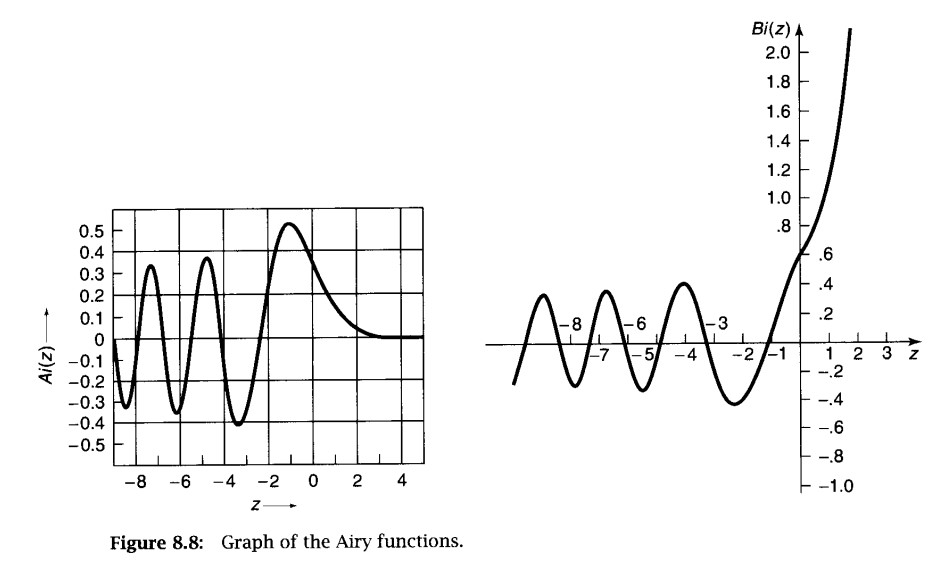
\includegraphics[width=10cm]{airyfunction.jpg}
	\caption{Airy Function}
\end{figure}

对波函数在转折点(E=V)处进行处理, “经典”区和“非经典”区在此处相接
透过处理这个方程可以(过程略,详细可参见\cite{griffiths_schroeter_2018}的8.3 THE CONNECTION FORMULAS)將 $E(z = 0)$ 表示為振幅為$E_{FS}$的入射波和具有相同振幅但相位偏移的反射波之和,即,
\begin{center}
    $\displaystyle E(z=0)=E_{\text{Fs}}\left[1+\exp-i\left(\frac{4}{3}\frac{\omega L}{c}-\frac{\pi}{2}\right)\right],$
\end{center}
这里$E_{FS}$是入射光波电场的自由空间的值,且$\varphi$只是一个相位因子且无法影响$|E|$,因此,
\begin{center}
    $\displaystyle E(\eta)=2\sqrt{\pi}\left(\frac{\omega L}{c}\right)^{1/6}E_{\text{FS}}e^{i\varphi}\mathbf{A}_i(\eta).$
\end{center}
图中可以看出电场的振幅在$\eta = 1$时可以达到最大值,即$(z-L) = -(\omega^2/c^2L)^{-1/3}$
\begin{center}
    $\displaystyle \left|\frac{E_{\max}}{E_{\text{FS}}}\right|^2\simeq3.6\left(\frac{\omega L}{c}\right)^{1/3}.$
\end{center}
因为驻波的形成,$E^2$的期望值增大四倍,这是因为介电函数变小和群速度变小。
接着,可以基于WKB理论获得峰值电场幅度的类似膨胀。 这里我们使用$k = \sqrt{\epsilon}(\omega/c)$和$|E| = E_{FS}/\epsilon^{1/4}$
随着$\epsilon$变小,波长变长。 
同样的,如果我们简单地减去$\pi/2$以说明临界密度表面的反射,则入射波和反射波之间的相移由 WKB 解给出。即
\begin{center}
    $\displaystyle \Psi=2\frac{\omega}{c}\int_{0}^{L}\sqrt{\epsilon}\mathrm{d}z-\frac{\pi}{2}=\frac{4}{3}\frac{\omega L}{c}-\frac{\pi}{2}.$
\end{center}

光波的磁场很容易从 E 的解中计算出来。注意到电矢量在 x 方向上并且波在 z 方向上传播,我们采用法拉第定律的 y 分量来获得
\begin{center}
    $\displaystyle B=-\frac{ic}{\omega}\frac{\partial E}{\partial z}.$
\end{center}即
\begin{center}
    $\displaystyle B(\eta)=-i2\sqrt{\pi}\left(\frac{c}{\omega L}\right)^{1/6}E_{\text{FS}}e^{i\varphi}\mathrm{A}_i'(\eta),$
\end{center}

这是一个非常棒的例子,不仅严格的按照WKB近似的步骤,并且非常合理的说明了波在等离子体中传播的问题。

\section{结论}
综上所述,WKB(Wentzel-Kramers-Brillouin)近似是一种强大的工具,用于解决量子力学中的薛定谔方程的近似解。
在均匀介质中,WKB近似已经得到广泛的应用,能够描述量子现象和波动行为。
WKB近似相对于其他精确的方法,WKB近似更简单、更直观,并且可以解决一些难以通过其他方法计算的问题。
然而,许多实际系统,像是是非均匀等离子体,具有空间上的变化性质,会需要解决更为复杂的物理行为。
通过WKB近似,我们可以得到非均匀等离子体中波的传播方程,并对物理运动进行定性描述;也可以更加全面的解释粒子散射的理论。

并且,WKB近似可以应用于解决类薛定谔的偏微分方程的近似解。将WKB近似扩展到非均匀介质,
特别是在非均匀等离子体中的应用,可以更准确地描述系统的性质和行为。尽管WKB近似在一些情况下存在局限性,
但它仍然是非常有用的方法。








\end{spacing}{}

\bibliographystyle{IEEEtran}
\bibliography{qp}

\end{document}